\documentclass[12pt,a4paper,titlepage]{report}

% Page setup
%
\usepackage{fancyhdr}
\pagestyle{fancy}
\fancyhead{}
\fancyfoot{}
\renewcommand{\headrulewidth}{0.4pt}
\setlength{\headheight}{15pt}

\lhead{\rmfamily \textcolor{gray}{\AcademicTitle}}
\rhead{\rmfamily \textcolor{gray}{\Report}}
\lfoot{\rmfamily \textcolor{gray}{\Author}{\StudentID}}
\rfoot{\rmfamily \thepage}


% Document Info
%
\newcommand\AcademicTitle{Optimising Test Runner Performance through Serverless Computing}
\newcommand\CommercialTitle{Bosco}
\newcommand\Author{Margaret McCarthy}
\newcommand\StudentID{20095610}
\newcommand\Date{March 2023}
\newcommand\Report{Project Report}
\newcommand\Stakeholder{ServisBOT Ltd.}
\newcommand\Course{Higher Diploma in Computer Science}
\newcommand\Reader{Supervisor: David Power}
\newcommand\University{South East Technological University}

\usepackage{Bosco}

\begin{document}

\pagenumbering{roman}

% title page 
\thispagestyle{empty}
\begin{center}
 \mbox{}\vfill
 {\fontsize{17pt}{20pt}\selectfont \bfseries \AcademicTitle}
 \vfill
 {\fontsize{14pt}{20pt}\selectfont \bfseries\itshape \CommercialTitle}
 \vfill
 {\fontsize{12pt}{20pt}\selectfont \bfseries \Report}
 \vfill
 {\fontsize{14pt}{20pt}\selectfont \bfseries \Author}
 \vfill
 {\fontsize{14pt}{20pt}\selectfont \bfseries \Stakeholder}
 \vfill
 {\fontsize{14pt}{20pt}\selectfont \bfseries \StudentID}
 \vfill
 {\fontsize{14pt}{20pt}\selectfont \bfseries \Reader}
 \vfill
 {\fontsize{14pt}{20pt}\selectfont \bfseries \Course}
 \vfill
 {\fontsize{14pt}{20pt}\selectfont \bfseries \University}
 \vfill
\end{center}
\clearpage

\tableofcontents

\listoftables

\listoffigures

% start of main matter
\clearpage
\pagenumbering{arabic}
\setcounter{page}{1}

\chapter{Introduction}

\section{Background}

The objective of this project is to create and execute a test runner for ServisBOT that focuses on specific features of the system, identifying those that are operational and those that are not. The proposed system has the working title Bosco.

ServisBOT is a company which specialise in chatbot technology and conversational AI. They provide customer service by allowing end users to communicate with a business or service through a pop up messenger on an online platform. 
The technology is cloud based and mostly serverless, it is provided over the internet rather than using storage on a physical computer or server. ServisBOT has a global customer base so the system has to be consistently monitored and so tests are run continuously to ensure any problems are detected and resolved immediately. 

Software testing is a critical element of software quality assurance and represents the ultimate review of specification, design and coding. Software testing is usually performed for one of two reasons: defect detection, and reliability estimation. \cite{Ahamed}

\subsection{Frankenstein}
The components of a chatbot and each of its functions are created using microservice architecture. This is an architectural style that structures an application as a collection of services that are:
\begin{itemize}
  \item Independently deployable
  \item Loosely coupled
  \item Organised around business capabilities
  \item Owned by a small team
\end{itemize}
The microservice architecture enables an organization to deliver large, complex applications rapidly, frequently, reliably and sustainably - a necessity for competing and winning in today's world. \autocite{Microservices}
There is a suite of tests which ServisBOT have named Frankenstein which run against these micro services testing every component of the chatbot. They run several times an hour, every hour. 
\subsection{TestCafe}
The tests use a software package called Testcafe which is used for automated browser testing.  By opening messenger in a browser in order to run the tests, it simulates what a user would do by interacting with a chatbot. If the chatbot reacts in the expected way the test passes, otherwise the issue is investigated and resolved.
\subsection{EC2}
The Frankenstein test suite is run on two EC2 instances in two different AWS regions. AWS Elastic Compute Cloud (EC2) is basically a virtual machine where developers can define the resources they need. For example, what regions the are to be run in. 
\section{The Issue}

Running the tests causes a lot of contention for CPU and memory. When a test run is instigated all tests are competing for CPU usage because each EC2 instance is running thirty plus tests on one server which has limited memory.

Also there are numerous problems with Testcafe. 
\begin{itemize}
 \item ServisBOT, when running the Frankenstein test suite, find Testcafe resource heavy, expensive and inefficient, causing slow CPU performance. 
 \item Because of the competing resources some tests affect the performance of others. 
 \item Debugging and monitoring of the tests is complex.
 \item The test suite does not scale. Scalability is essential in order to increase the number of tests according to the number of user interactions and alternatively to reduce the number of tests when interactions drop which would not only prove to be more cost effective but would mostly solve all the issues mentioned.
\end{itemize}

 \begin{figure}[ht]
  \centering
  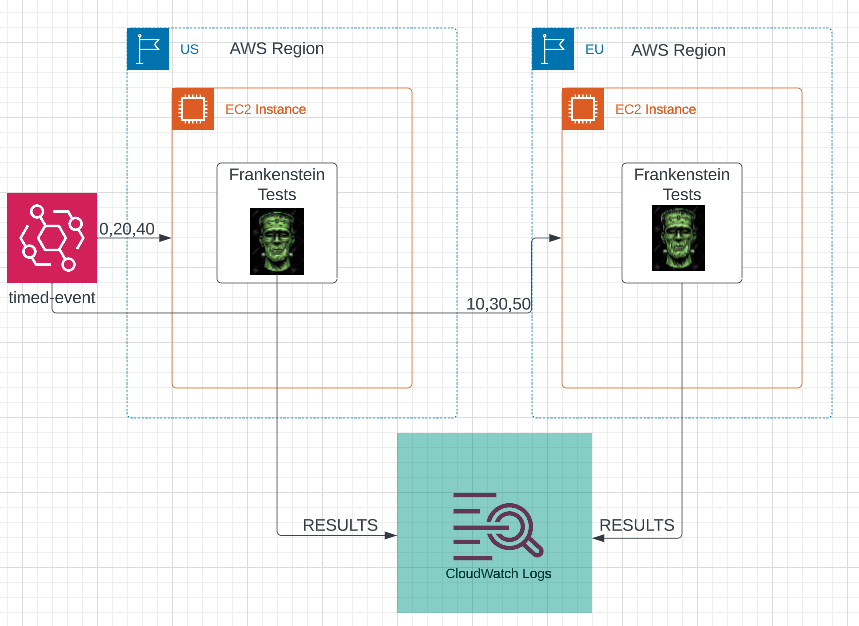
\includegraphics[width=\textwidth,height=\textheight,keepaspectratio]{./diagrams/frank_high_level.png}
  \caption{High level view of Frankenstein}
 \end{figure}
 \clearpage

\section{Purpose and Requirements for Bosco}

The objective of this project is to create a new test runner, Bosco, that is more efficient, scalable, optimised, and cost-effective than Frankenstein. 
The purpose is to completely revamp the existing test suite and develop AWS Lambda functions that can run each test independently without memory competition. 
By doing so, the test suite could be scaled infinitely, perform faster, and potentially be more cost-effective. 
Each test will eventually be migrated from Frankenstein to Bosco once the infrastructure has been developed.

In particular the migration will focus on an automation tool called Puppeteer which has been proven by ServisBOT to be more performant than Testcafe. The Puppeteer package includes its own browser, Chromium, whereas Testcafe launches an external browser which is slow and cumbersome. With Puppeteer there is more control over what the developer can test, it is more efficient, easier to debug and has a lot more functionality. It is widely chosen by developers now. (4.6 million weekly downloads, 2023-03-02) \cite{Puppeteer}

\begin{figure}[ht]
 \centering
 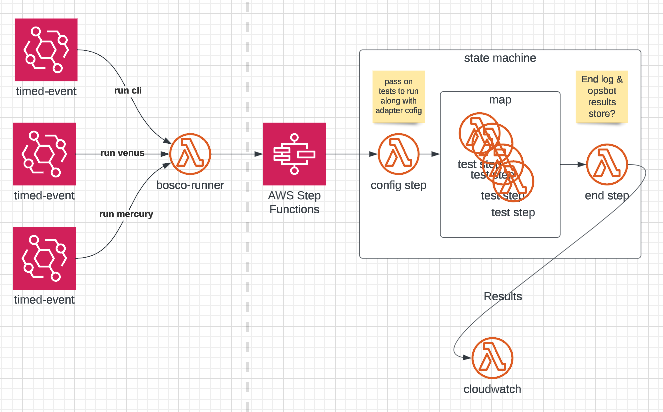
\includegraphics[width=\textwidth,height=\textheight,keepaspectratio]{./diagrams/bosco_high_level.png}
 \caption{High level view of Bosco}
\end{figure}

\chapter{Research and Development}

In order to determine the best approach, technologies and methodology for Bosco, it was concluded that the research and analysis phase necessary for the implementation of this project was the following:

\begin{itemize}
 \item Cost Analysis of Frankenstein
 \item Research into possible testing frameworks for Bosco
 \item Puppeteer comparison to Testcafe
 \item Lambda vs EC2 comparison
 \item Possible implementations and modelling of Bosco
 \item Additional requirements for implementing Bosco
 \item Scope of the project
\end{itemize}

\section{Cost Analysis of Frankenstein Tests}

The following cost analysis was carried out on Frankenstein. There is two EC2 instances running the tests in the EU and the US costing ServisBOT on average \$20 per day for each region. This costs the company almost \$15,000 a year to run tests.

\begin{figure}[ht]
 \centering
 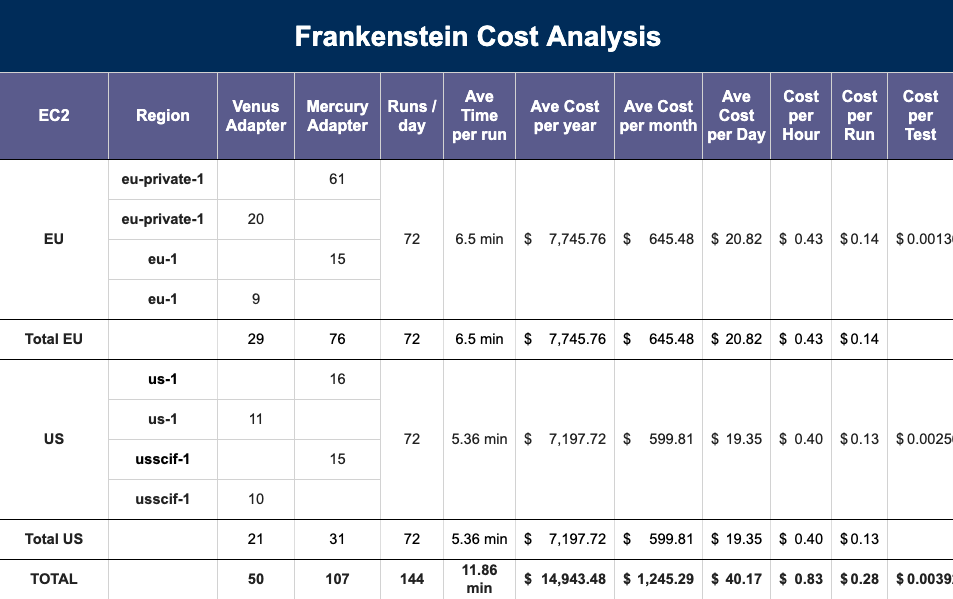
\includegraphics[width=\textwidth,height=\textheight,keepaspectratio]{./diagrams/frank_cost_analysis.png}
 \caption{Frankenstein Cost Analysis}
\end{figure}

\section{Research into Possible Testing Frameworks for Bosco}

Frankenstein uses Mocha as its testing framework but there are multiple frameworks that ServisBOT could choose from. The following is an investigation into what else is available as well as a review of the current framework, Mocha.
\subsection{Mocha}

According to Mocha documentation, Mocha is a feature-rich JavaScript test framework running on Node.js and in the browser, simplifying asynchronous
testing. Mocha tests run serially, allowing for flexible and accurate reporting, while mapping uncaught
exceptions to the correct test cases. \autocite{Mocha}

Asynchronous testing is a technique used in software testing to verify the behavior of code that relies on asynchronous programming or event driven architecture. Asynchronous programming allows the program to perform tasks concurrently or in parallel, rather than waiting for each task to complete before moving on to the next one. 

Mocha provides functions that execute in a specific order, logging the
results in the terminal window. Mocha also cleans the state of the software being tested to ensure that test
cases run independently of each other.

\begin{figure}[ht]
 \centering
 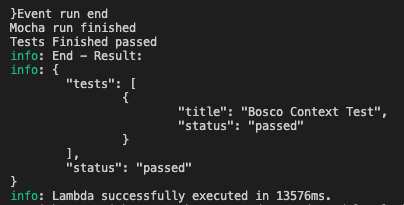
\includegraphics[width=0.75\textwidth,height=0.75\textwidth,keepaspectratio]{./diagrams/mocha_test_result.png}
 \caption{Mocha Test Result Output}
\end{figure}

\subsection{Jest}

Jest is a JavaScript testing framework created by Facebook. It is open source, well-documented and popular due to its
high speed of test execution. It comes with a test runner, but also with its own assertion and mocking library unlike Mocha where you need to install an assertion
library, there is no need to install and integrate additional libraries to be able to mock, spy or make assertions.

\subsection{Mocha vs Jest}

\begin{table}[ht]
 \centering
 \small
 \setlength\tabcolsep{6pt}
 \begin{tabular}{|c|c|c}
  \hline \textbf
  {Mocha}       & \textbf {Jest}\\
  \hline\hline
  Flexible configuration options & High Speed of Test Execution\\
  \hline
  Good Documentation       & Good Documentation\\
  \hline
  Ideal for back-end projects  & Test Runner included\\
  \hline
  Ad-hoc library choice     & Built in assertion and mocking library\\
  \hline
 \end{tabular}
 \caption{Mocha Vs Jest}
\label{table:mocha:jest}
\end{table}

\section{Review of Puppeteer}

Puppeteer is a popular test automation tool maintained by Google. It automates Chrome and Firefox and is relatively simple and stable to use.
Fundamentally Puppeteer is an automation tool and not a test tool. 
This means it is incredibly popular for use cases such as web scraping, generating PDFs, etc. \autocite{PuppvsSel}

Testing user flows within web applications usually involves either using an automated headful
browser (i.e. FireFox with Selenium) or a headless browser, one that presents no UI, that is built on top of its own unique JavaScript
engine (i.e. Testcafe). This creates a situation where trade offs have to be made such as speed vs reliability.
Puppeteer aims to remove this trade off by enabling developers to leverage the Chromium browser environment
to run their tests and by giving them the flexibility to leverage headless or headful browsers that run on the same underlying platform as their users. \autocite{Crowther}

\subsection{Pros of using Puppeteer}

\begin{itemize}
 \item Simple to set up.
 \item Good documentation with lots of tutorials.
 \item Promise based which allows for management of asynchronous code.
 \item Programmable web browser.
 \item Installs Chrome in a working version automatically.
 \item Puppeteer has a thin wrapper which provides a simpler interface for an underlying complex system.
 \item Bi-Directional (events) \- automating console logs is easy.
 \item It uses JavaScript first, which is one of the most popular programming languages.
 \item Puppeteer also gives you direct access to the Chrome DevTools Protocol which allows for developers to feel like there are fewer moving parts.
 \item Works with multiple tabs and frames. It has an intuitive API
 \item Trusted Actions: This criterion means dispatching events by the user which allows for user behaviours like hovers.
 \item End to end tests are very fast in practice but people suffer misconceptions regarding the execution speed. Typically, it's the website or web-app that are slow and the tests end up waiting for the web app to be ready most of the time.
 \item Pro and Con: Stability, which means how often tests fail after being authored other than when detecting a real application bug. Puppeteer waits for certain things but has to wait manually for others. 
 \item Debugging: Can write and debug Javascript from an IDE\@.
\end{itemize}

\subsection{Cons of using Puppeteer}
\begin{itemize}
 \item Limited cross-browser support. Only Chrome and Firefox.
 \item Feels like an automation tool and not a test framework. Often developers have to re-implement testing-related tools.
 \item Grids (running concurrently) in production are often a challenge
 \item The automatic browser set-up, downloads Chromium and not Chrome and there are subtle differences between the two.
 \item Smarter Locators: No support for selecting elements in multiple ways.
 \item Does not support parallelism, grids and infrastructure.
 \item Does not support self healing tests and automatically improving tests.
 \item Does not support Autonomous testing which is testing without code or user intervention.
\end{itemize}

\subsection{Testcafe}

TestCafe is a Node.js tool to automate end-to-end web testing. It runs on Windows, MacOs, and Linux and
supports mobile, remote and cloud browsers (UI or headless). It is also free and open source.

\begin{table}[ht]
  \centering
  \small
  \setlength\tabcolsep{6pt}
  \begin{tabular}{|c|c|}
   \hline \textbf
   {Pros} & \textbf {Cons}\\
   \hline\hline
   Cross Browser Testing&Expensive\\
   \hline
   Open Source& Slow\\
   \hline
   Easy Setup \& Installation& Difficult to debug\\
   \hline
   Built-In Waits& No browser control\\
   \hline
   Supports devices without extra software package & Simulated events leads to false positives\\
   \hline
   UI End to End Testing\\
   \hline
   Both client and server side debug \\
   \hline
  \end{tabular}
  \caption{Pros and Cons of Testcafe}
 \end{table}

\begin{figure}{h}
 \centering
 \subfloat[\centering Npm Downloads]{{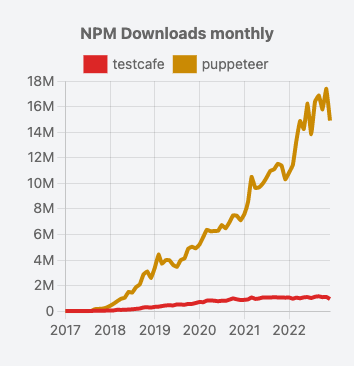
\includegraphics[width=5cm]{./diagrams/npm_pupp_tc}}}
 \qquad
 \subfloat[\centering GitHub stars]{{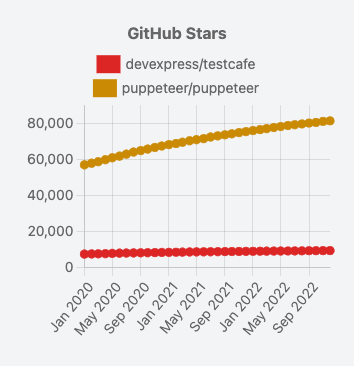
\includegraphics[width=5cm]{./diagrams/github_stars}}}
 \caption{Puppeteer vs Testcafe NPM statistics}
\end{figure}

\section{EC2 vs Lambda comparison}

AWS Elastic Compute Cloud (EC2) is basically a virtual machine called an instance. Users can create an instance and define
the resources neccessary for the task at hand. For example the type and number of CPU, memory, local storage and scalability. EC2 instances
are intended for consistent, static operations and users pay a recurring monthly charge based on the size of the instance, the operating
system and the region. The instances run until they are deliberately stopped.

Lambda on the other hand is billed per exectution and per ms in use with the amount of memory the user allocates to the function.
When a lambda funciton is invoked, the code is run without the need to deploy or manage a VM\@. It is an event based service that is
designed to deliver extremely short-term compute capability. AWS handles the back-end provisioning, loading, execution, scaling and unloading of the user's code.
Lambdas only run when executed yet are always available. They scale dynamically in response to traffic.

\begin{table}[ht]
  \centering
  \small
  \setlength\tabcolsep{6pt}
  \begin{tabular}{|c|c|c|}
   \hline
   \textbf{Feature} & \textbf{Lambda} & \textbf{EC2}\\
   \hline\hline
   Time to execute&milliseconds&seconds to minutes\\
   \hline
   Billing increments& 100 milliseconds&1 second\\
   \hline
   Configuration \&Function& Operating System\\
   \hline
   Scaling Unit&Parallel function executions&Instances\\
   \hline
   Maintenance& AWS&AWS and User\\
   \hline
  \end{tabular}
  \caption{Comparison of AWS Lambda and EC2 \autocite{inbook}}
 \end{table}

\section{Conclusion}
Based on the research and analysis conducted, it can be affirmed that ServisBOT's decision to use Puppeteer in conjunction 
with Mocha instead of Testcafe is affirmed. Puppeteer will give the developers more control over the tests, testing will be more reliable 
and easier to use and debug. Together with migrating the test runner from EC2 to Lambda, the test suite will become infinitely scalable and 
more cost efficient. A revamp of the test runner will mean that issues encountered by Frankenstein can be resolved and unnecessary costs (for 
example running too many tests) can be eliminated.

\chapter{Initial Design \& Implementation}

\section{Proof of Concept - Running Puppeteer on a Lambda}

In order to prove it is possible to run Puppeteer tests on AWS Lambda, a basic end to end test was designed
to run with Puppeteer. This automated a scenario whereby a browser, Chromium was launched with the url of the
messenger page. After the page loaded, the messenger button was toggled and the chatbot would load. The test
passed if the text from the messenger returned the expected output text.

\subsection{Mocha}

Mocha was incorporated as the testing framework. Assertions are made using the Assert library package and logged to the console but it is not in essence a testing tool.
Once mocha was configured and run without errors the next step was to run the script in a lambda.

\begin{figure}[H]
 \begin{tcolorbox}
  \begin{minted}[breaklines]{javascript}
  // basic-puppeteer.js
  const puppeteer = require('puppeteer');
  const url = 'https://www.google.com';
  async run () => {
   const browser = await puppeteer.launch();
   const page = await browser.newPage();
   await page.goto(url);
   await page.screenshot({path: "screenshot.png"});
   browser.close();
  }
  run();
\end{minted}
\end{tcolorbox}
\captionof{figure}{Example of a function written with Puppeteer which takes a screenshot of the Google homepage and stores it locally}
\end{figure}

However, there are problems running Puppeteer in a lambda. Lambda has a 50 MB limit on the zip file you can upload. 
Due to the fact that it installs Chromium, the Puppeteer package is significantly larger than 50 {MB}. This 
limit does not apply when uploaded from an S3 bucket but there are other issues. 
The default setup of some Linux distributions, including the ones used by AWS Lambda do not include the necessary libraries required to allow Puppeteer to function.

\subsection{Node Modules}

A developer named Hansen\autocite{Hansen}, figured out a work-around for this in the form of the node modules, \textbf{puppeteer-core} and \textbf{chrome-aws-lambda}.
Both these modules installed allow for a version of Chromium that is built to run for AWS Lambda. Incorporating
these ensures the tests run successfully. Unfortunately these modules need to be in parody with each other.

The aws-chrome-lambda module has not been updated since June 2021 so its latest version is 10.1.0 whereas
puppeteer-core has been updated regularly and at time of writing (26/03/23) is at version 19.8.0. When the version numbers are
synced the lambda function passes. Therefore using the latest version of both modules would mean they are incompatible with each other.
Whatever the reason for these modules not being updated, relying on them is impractical and will eventually lead to the tests being broken.

\subsection{Docker}
 
A Docker container was used instead of node modules to condense the code. A Docker
container is a standalone piece of software that packages up code and all its dependencies so the application runs quickly and reliably from one computing environment to the next.
A Docker container image is a lightweight, standalone, executable package of software that includes everything needed to run an application: code, runtime, system tools, system libraries and settings.
Container images become containers at runtime. When you use a Docker container, it creates an isolated environment that shields the application from other parts of the computer it is running on. This 
means that the application can work smoothly and consistently, even if it is being used in different stages of development or on different computers with different settings.

\begin{figure}[H]
  \centering
  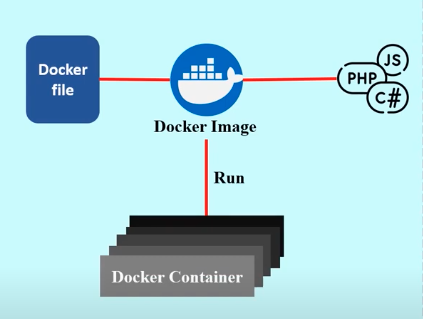
\includegraphics[width=10cm]{./diagrams/dockerexplained.png}
  \captionof{figure}{Illustration of Docker}
 \end{figure}

\subsection{Conclusion}
The puppeteer test was run locally using a Docker engine. When the test was functioning as expected the docker image got built, tagged and pushed to an AWS repository. 
The latest Docker container image was deployed to the Bosco test-runner Lambda container where it was run and tested in a Lambda environment.
This significantly sped up the testing process, automating a browser in milliseconds compared to the previous method's average time of six seconds.
The process provides more control over the testing environment and successfully runs the tests by targeting specific tests through the event handler input parameters.
The results validate the feasibility of running tests in a Lambda environment using Puppeteer.

\section{Initial Stepfunction Research and Development}

The use of a Step Function in order to run the tests had been considered by ServisBOT to be a viable option for Bosco. With 
step functions a workflow can be created through a series of lambda functions with each step being a state within
the workflow. They are based on a state machine and tasks, where a state machine is a workflow and a task is a
state in that workflow that another AWS service performs.

\begin{figure}[H]
 \centering
 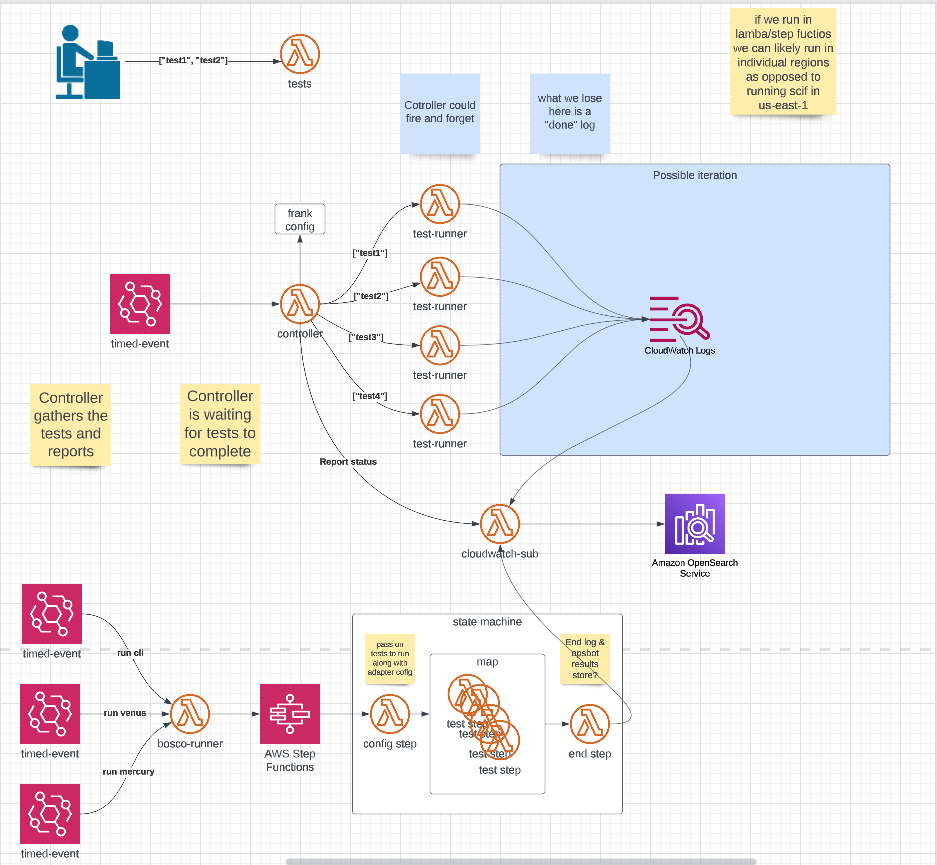
\includegraphics[width=15cm]{./diagrams/possible_implementation}
 \captionof{figure}{Bosco Initial Possible Implementations}
\end{figure}

\section{State Machine Transitions}

The Bosco test suite runs through 5 state transitions (Start, StartState, Map, Done, End) plus an additional transition for each test run (Running). With three tests, there are eight states as the \textbf{Running} state is executed three times. The first state is the \textbf{Start} state which initiates the run and then the \textbf{StartState} is invoked, creating an array of tests and passing the payload to the \textbf{Map} state.

This experiment focuses on using the Inline Map state instead of the Distributed Map state. The Inline Map state is used for fewer than forty parallel iterations which is appropriate for the number of tests that Bosco will run, while the Distributed Map state is used for larger workloads. 
The map state can run a lambda for each test, or it can run an array of tests. The lambdas run in parallel with each other with the results of the tests outputted to the \textbf{Done} lambda, the next state, which processes and runs the tests. Finally, a state prints out the results and the \textbf{End} state completes the workflow.

\begin{figure}[H]
 \centering
 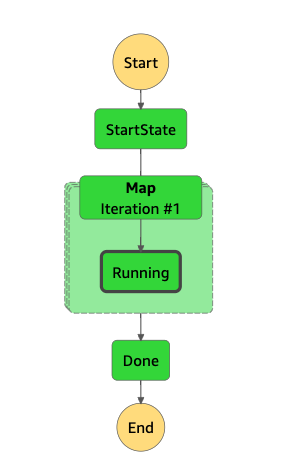
\includegraphics[width=5cm]{./diagrams/step_function}
 \caption{Bosco State Machine}
\end{figure}

\begin{figure}[H]
 \centering
 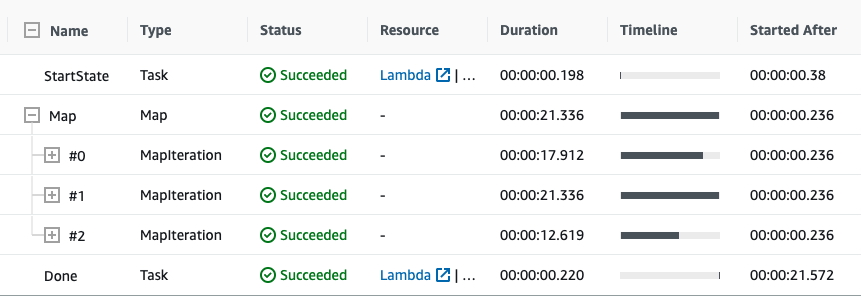
\includegraphics[width=15cm]{./diagrams/tablestepfx.png}
 \caption{Results of Execution of State Machine}
\end{figure}

\subsection{Cold vs Warm Lambdas}

Comparisons were made between running the tests on cold lambdas as opposed to warm lambdas and the results were significantly different. The cold lambda run ran in 40 seconds and the warm lambda run ran in 14 seconds total which is more than half the duration. 
Later in the project imiplementation, an issue occured with Lambda, where the caching of files was occuring which is why a warm run is quicker than a cold run. This was not the intention and it caused the tests to fail. 
This means testing the code locally is not always compatible with testing it in a lambda environment. When the code passed through the CICD process it fell over in the Lambda environment and the code needed to be refactored to take this into consideration.

\subsection{Initial Cost Analysis of Bosco Step Function State Machine}

The cost of running the test suite in a state machine using AWS Step Functions was based on the number of state transitions.\autocite{Amazon} 
This cost analysis does not account for error handling, which may increase the cost due to retries. The cost per transition is \$0.000025 according to the AWS pricing calculator. 
The analysis is based on the current number of tests and the frequency they are run (three times an hour), which at the time of conducting the cost analysis may vary for Bosco tests.

\begin{figure}[H]
 \centering
 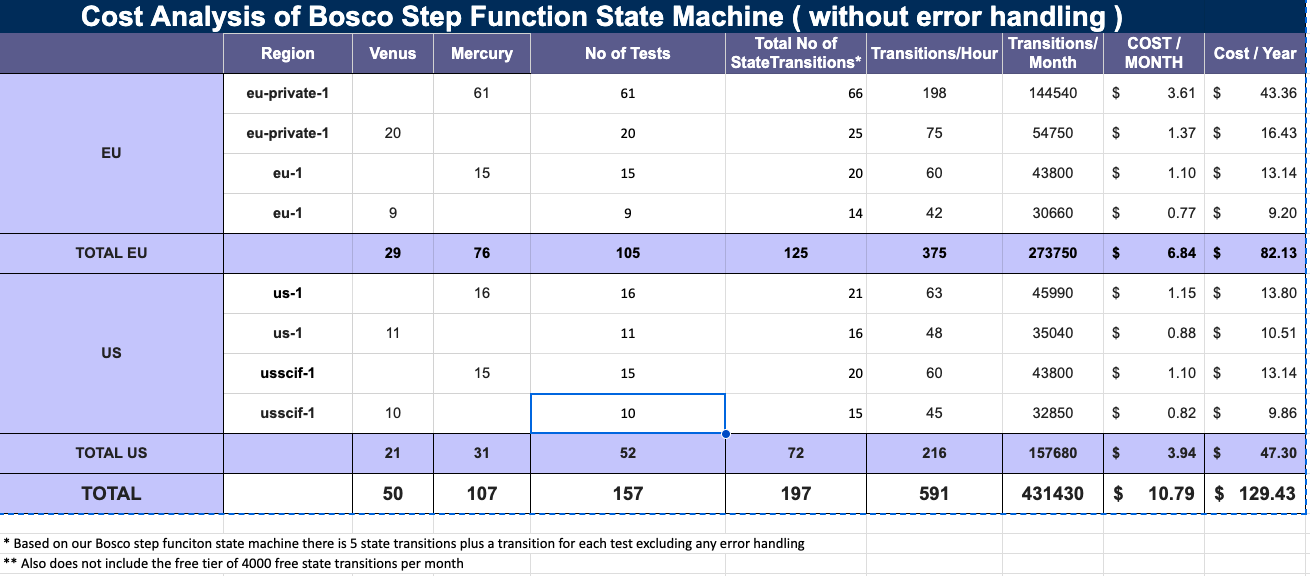
\includegraphics[width=15cm]{./diagrams/sfcost}
 \caption{Bosco Step Function Cost Analysis}
\end{figure}

\chapter{Bosco Implementation}
\section{Lightning Page}
The implementation of Bosco began after finalising the proof of concept. 
The first step involved creating a Lightning page class which is the page the tests are running against. 
The class serves as the source for accessing the selectors and functions that have been added specifically for the Lightning page. 
Confining this functionality to a class reduces boilerplate code which is repetitious code.

\begin{figure}[H]
 \begin{tcolorbox}
  \begin{minted}{js}
  async getMessage(index) {
    const allMessages = await this.getAllMessages();
    return allMessages[index];
  }
  \end{minted}
 \end{tcolorbox}
 \caption{Example of getMessage Lightning Page function}
\end{figure}

With this starting point the interaction node test was refactored to use the Lightning page. Two functions were
created, one which clicks through the selectable list and another function which types into messenger instead of
clicking the list. A BrowserFactory class was created which has a function to create the browser.

\section{Tests}
\subsection{Context Test}
The first actual Frankenstein test to be converted to Bosco was the Context test. This test sets the context from the url
and tests if it is outputted with the rest of the context to the messenger. Working through this test exposed a bug in the Frankenstein test. 
It was not testing what it was supposed to be testing even though the test was passing. Once the error was highlighted and fixed by the developer team it was now possible to finish writing the test
and ensure it was working correctly. 

\subsection{Conversation Engaged Test}
The next test was the Conversation Engaged test. Whenever a user interacts with a bot, a goal is generated, which is a default or custom event that's tracked to measure the success of the bot's interactions.
At first, it was believed that this test would be simple, but changes were requested after a pull request was submitted for review, including removing nested if statements and improving the code's formatting.

This created a need to parse the exported goal JSON result. However, an error was encountered in the Servisbot CLI proxy, where the outputted JSON was not formatted correctly and could not be parsed. 
To work around this, the CSV output option was used instead of JSON and the csv-parse node module was imported.

\subsection{Interaction Test}
% // TODO

\section{CloudFormation}
When deploying Bosco, a  CloudFormation template in the form of YAML is run.  CloudFormation is an AWS service that allows developers to define and deploy infrastructure as code.
The Cloudformation template, which can be in either YAML or JSON format, is used to define and provision the AWS resources. When the CloudFormation template is uploaded to AWS it 
creates a CloudFormation stack which is a collection of AWS resources that can be managed as one unit. 
The template specifies the necessary environment variables, parameters, conditionals and other resources such as IAM roles and policies. 

CloudFormation saves time and reduces errors as the same resources can be created multiple times once the template is defined.
A YAML formatting extension from Redhat to format the YAML file was used for Bosco as it is not possible to deploy the YAML unless the formatting is accurate.

Bosco's CloudFormation Template consists of the following resources:

\begin{description}
  \item [LambdaRole]: IAM (Identity and Access Management) role in AWS that is used to grant permissions to AWS Lambda functions.
  \item [ScheduledEventIAMRole]: IAM role used to grant permissions to the cron in Cloudwatch Events that will run the state machine.
  \item [BoscoIAMManagedPolicy]: AWS managed policy that defines the permissions for the roles and users attached to the IAM role.
  \item [ApiLambda]: The Lambda function that serves as an API endpoint for retrieving test run results from DynmaoDB.
  \item [TestOrchestrationLambda]: The Lambda function that configures the input to the state machine based on the profile provided in the event.
  \item [TestRunnerLambda]: The Lambda function that runs the suite of tests and returns the results.
  \item [TestResultsLambda]: The Lambda function that processes, stores and logs the tests results.
  \item [StateMachine]: The AWS Step Function State Machine that is used to manage the orchestrator, runner and results Lambdas in a workflow based on a map inline state. 
  \item [ApiGateway]: The API Gateway created to access the DynamoDB results table.
  \item [ResultsDynamoTable]: The DynamoDB table that the results are written to.
  \item [S3BucketScreenshots]: The S3 bucket that screenshots of failed tests are stored in.
\end{description}

\section{Environment Variables}
The environment variables are made up of the credentials needed to log into the ServisBOT CLI, the Log Level and the SSM credentials for the Lex V2 test which uses an external service.  
Storing the log level in the environment variables allows for consistency across the application, better security, easier debugging and flexibility. 
The log level can be changed without changing the code.

Initially, the environment variables were passed to the Orchestrator through the event. Once this was working, the environment variables became part of the profile. However, a more 
secure option was neccessary so they were subsequently removed from the profile and stored in AWS Systems Manager Parameter Store, an AWS service for storage, configuration, secrets and data management. 

Two more classes were constructed in addition to the Environment class in order to resolve the environment variables. 
\begin{description}
  \item[EnvironmentResolver:]A class with three functions: resolveEnvironment; resolveEnvironmentVariable; retrieveSSMParam
  \item[resolveEnvironmentVariables:]A class which takes in the test profile and uses this to return an array of environment variables.
\end{description}

\begin{figure}[H]
  \begin{tcolorbox}
   \begin{minted}{json}
    "environment": [
      {
        "name": "SB_CLI_CREDENTIALS",
        "value": {
          "username": "some-username",
          "password": "some-password"
        }
      },
      {
        "name": "LEX_V2_CROSS_ACCOUNT_ROLE_SECRET",
        "value": {
          "externalId": "some-externalId",
          "crossAccountRole": "some-cross-account-role"
        }
      },
      {
        "name": "LOG_LEVEL",
        "value": "INFO"
      }
    ],
 \end{minted}
  \end{tcolorbox}
  \caption{Environment Variables Inputted to Handler}
 \end{figure}

The environment variables are provided to the handler at the same level as the testSuite and the testProfileConfig. 
By fetching and resolving the environment variables in the Orchestrator, this allows for a shared environment between the tests rather 
than providing the environment to each test which would be inefficient and resource heavy. Environments can grow and so this allows 
for flexibility in the development of Bosco.

It was essential to prove it was possible to flip between environments by either providing the environment to the
Orchestrator Lambda or by inputting it to the State machine as an event. 
This was important to prove because providing the state machine with the environment variables and testSuite configuration there is more control over the state
machine. What tests are run with what environment variables can be determined at any stage.

The state machine was then refactored to use a shared environment instead of
passing the environment variables in with each test object. In the state machine definition there is an option to
use an ItemSelector which allows the map to iterate over the ItemsPath but use the ItemSelector to add additional
parameters.

The updated definition of the state machine included the following extra parameters:

\begin{figure}[H]
 \begin{tcolorbox}
  \begin{minted}{json}
  {
    "ItemsPath":"$.testSuite",
    "ItemSelector": {
      "testSuite.$": "$$.Map.Item.Value",
      "environment.$": "$.environment",
      "testProfileConfig.$": "$.testProfileConfig",
      "executionId.$": "$$.Execution.Id"
    },
  }
\end{minted}
 \end{tcolorbox}
 \caption{State Machine Definition passing the environment to the Handler}
\end{figure}

The input to the Handler became the following:

\begin{figure}[ht]
 \begin{tcolorbox}
  \begin{minted}{json}
    {
      "testProfileConfig": {
        "..."
      },
      "executionId": "...",
      "environment": [
        "..."
      ],
      "testSuite": {
        "tests": [
          {
            "path": "goals/puppeteer-conversation-engaged.js"
          }
        ]
      }
    }
\end{minted}
 \end{tcolorbox}
 \caption{Input to one Iteration of Map State with just the Test Path}
\end{figure}


\section{Test Profiles}
One significant way in which Bosco will differ to Frankenstein is in the capability to run test profiles rather than 
running all the tests, all the time, in all the regions. By creating a test profile it is possible to specify which 
environment, region and frequency of the tests which Frankenstein does not have the ability to do. 

A profiles folder was created with two different profiles for the adapters Venus and Mercury in the dev environment. Each profile 
contained the test suite so the orchestrator needed to be updated in order to read the file paths from the JSON provided in the 
event profile. The node module \textbf{file system\&(fs)} was used to read the contents of the profile, this was parsed to 
a javascript object and a spreader operator was used to combine the contents of the profile and the contents of 
the even inputted to the orchestrator and output these to the handler.

\begin{figure}[H]
 \begin{tcolorbox}
  \begin{minted}[breaklines]{javascript}
  const readProfile = fs.readFileSync(testProfile, (err, data) => {
  if (err) throw err;
   logger.info(data);
  });
  const profile = JSON.parse(readProfile);
  const output = { ...profile, ...event };
  \end{minted}
 \end{tcolorbox}
 \caption{Parsing a JSON string to a javascript object and use of the spreader (\dots) operator}
\end{figure}

Next the global environment variables were removed so instead of reading them from the input to the orchestrator they would 
be passed from the profile to the tests. There was quite a lot of code build needed for this as Mocha is limiting in that it doesn't 
allow the passing of parameters to the tests. 

\subsection{Singleton Class: TestRunnerConfig}
A singleton class was created to overcome this. A siingleton class is a class that can only have one instance of 
itself. It is used when there is going to be no change or update to the object for the duration it is used. This would be the case with our tests as we would just be using the configuration for accessing the lightning page to run the tests.

Initially the TestRunnerConfig took in the runnerEvent and created an instance of itself. It had getters to get different variables from the event which at the time were just the profile, testConfig, testSuite and environment. The tests ran but now the aim was to remove process.env to set the variables and use an Environment class that instead reads the environment variables from the TestRunnerConfig.

An Environment object was created using the environment from the event. This could now be accessed in the tests by calling the getters from the Environment object.
\begin{figure}[H]
 \begin{tcolorbox}
  \begin{minted}[breaklines]{javascript}
const testRunnerConfig = TestRunnerConfig.getInstance();
const environment = testRunnerConfig.getEnvironment();
const params = {
organization: environment.getOrganization(),
username: environment.getUsername(),
password: environment.getPassword(),
region: environment.getSBRegion()
};
\end{minted}
 \end{tcolorbox}
 \caption{Replacing proccess.env with getters to an Environment class invoked by a singleton class, TestRunnerConfig}
\end{figure}

\section{Endpoint Proxy}

Bosco needed to support both Mercury and Venus engagement adapters similar to Frankenstein. This is achieved through the endpoints whereby 
each endpoint is suffixed by the test profile name. When the endpoint is created instead of creating it uniquely with the timestamp, middleware 
in the form of an Endpoint proxy would instead suffix the endpoint with the profile and thereby point the tests to the url 
containing the endpoint proxy. To prove the tests were making network calls to either Mercury or Venus, the tests were slowed down, run in headful mode and 
the network tab examined. When the browser was talking to Venus there calls to \textbf{VendAnonConversation} and \textbf{ReadyForConversation} and when there were calls to Mercury, \textbf{graphql} calls were evident.

\begin{figure}[H]
 \centering
 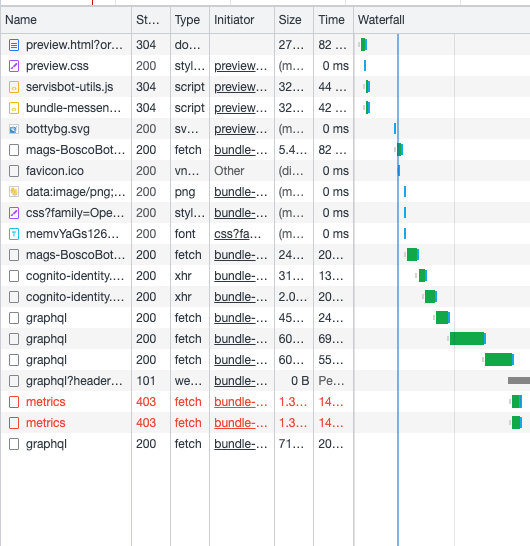
\includegraphics[width=15cm]{./diagrams/mercury_network_calls.png}
 \caption{Mercury Network Calls}
\end{figure}

\begin{figure}[H]
 \centering
 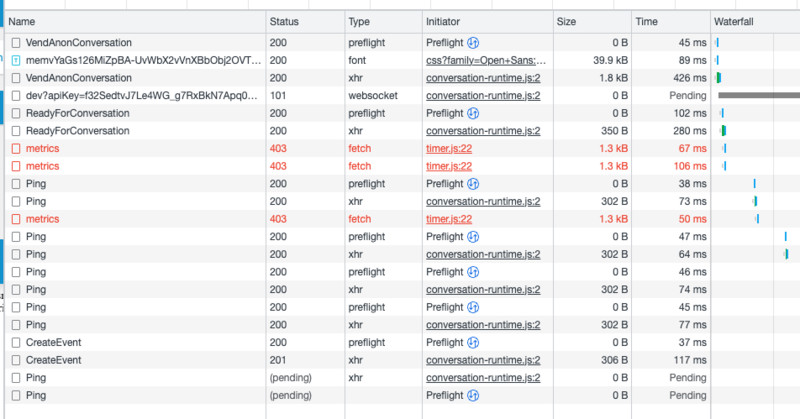
\includegraphics[width=15cm]{./diagrams/venus_network_calls.png}
 \caption{Venus Network Calls}
\end{figure}

\section{Creating a Test with a Secret}
Many of the Frankenstein tests use secrets in order to run the tests. Secrets can be defined as secure documents containing access keys, api keys, api secrets or IDs to external systems. They can be created and stored in the ServisBOT system and then referenced by bots securely. 
This is how ServisBOT manage API keys for AWS\@.

The test that was chosen was the NLP worker, Lex V2, intent-publish test. A \textbf{Lex} worker is a remotely managed NLP worker who takes input and sends it to a Lex bot for Natural Language Processing. A Lex bot is an Amazon bot, users use ServisBOT to access, manage and run their Lexbots. 
\textbf{NLP} is a form of Artificial Intelligence that transforms text that a user submits into language that the computer programme can understand. In order for ServisBOT to classify utterances using a remote managed NLP, the correct API keys, access tokens or cross account roles need to be configured in the ServisBOT Secrets Vault.

An AWS cross account role, ie a secret, is required in order to access Lex. An environment variable was created that the test could access called LEX\_V2\_CROSS\_ACCOUNT\_ROLE\_SECRET and to this was assigned the secret definition for dev in JSON format. 

This test creates a long living bot which is a bot that is not deleted after the test but is created the first time the test is run and then reused for every test. The bot's variable intent is updated with the timestamp every time to ensure the bot is publishing successfully. When the bot is publishing its status is polled every 5 seconds and when published its status is SUCCEEDED and so the test starts.

A bot class was created so that a publish function which polled the status of the publishing and outputted the status to the console could be created. This was so 
the test behaved the same way as Frankenstein but also because using the ServisBOT cli proxy does not have this functionality so in calling sbCli.publish we would 
not have the polling outputted to the console.

\begin{figure}[H]
 \centering
 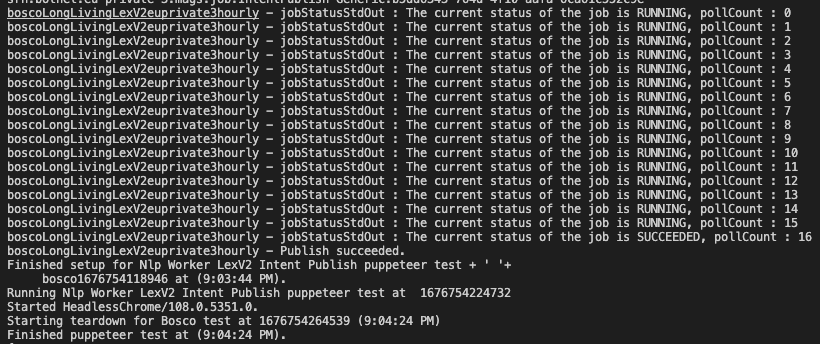
\includegraphics[width=15cm]{./diagrams/nlp_worker_poll.png}
 \caption{NLP worker test with polling}
\end{figure}

\section{SSM Parameters}
The next task for Bosco was to build the environment in the orchestrator using SSM parameters. 
SSM (Systems Manager) is a service provided by AWS that allows you to securely store and retrieve data for your application \cite{Halley}.
They can be encrypted and the service is easy and free to use. 
A few lines of code can retrieve the parameters from the store. 

The steps to this task were as follows:
\begin{itemize}
\item The parameters were created in the SSM parameter store in the same format as the Frankenstein parameters.
\item Code was added to the orchestrator to read the SSM parameters using the node module \textbf{aws-sdk}.
\item A new policy was added to the  CloudFormation template in order to give IAM permissions to read from the parameter store
\item The environment was built in the orchestrator by retrieving the ssm parameters in the orchestrator, building the envirnoment object and returning this to the output.
\item A new class, Secrets was added in order to retrieve the SSM parameters from the parameter store to extract that work from the orchestrator. Later to be renamed EnvironmentResolver. This was done by passing the ssm through to the Secrets constructor.
\item The README was updated to reflect the changes.
\end{itemize}

\begin{figure}[H]
 \centering
 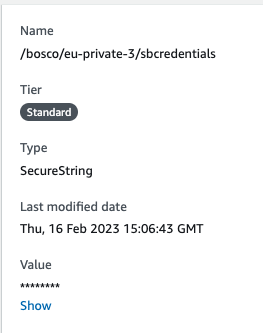
\includegraphics[width=8cm,height=8cm,keepaspectratio]{./diagrams/ssm_params.png}
 \caption{SSM Parameters created in AWS Systems Manager}
\end{figure}

\section{Eventbridge Rules (CRON) }

Like Frankenstein, Bosco needs to run on a scheduled event. WS Eventbridge allows developers to trigger evAents on a CRON which is `a command to an operating system or server for a job that is to be executed at a specified time`. 
To trigger the state macine to run different profiles at different times, in different regions the  CloudFormation file needed to be updates. 
\begin{itemize}
 \item First the rule defaults were added to the  CloudFormation
 \item The CRON rules were then added 
  \begin{tcolorbox}
   \begin{minted}[fontsize=\footnotesize, breaklines]{yaml}
   ScheduleMercuryExpression: { Type: String, Default: "cron(0,20,40 * * * ? *)" } # run at 0,20,40 past the hour
   ScheduleVenusExpression: { Type: String, Default: "cron(10,30,50 * * * ? *)" } # run at 10,30,50 past the hour
   ScheduleHourlyExpression: { Type: String, Default: "cron(0 * * * ? *)" } # run at 0 past the hour
   \end{minted}
  \end{tcolorbox}

 \item The triggers were added.
 \begin{tcolorbox}
  \begin{minted}[fontsize=\footnotesize, breaklines]{yaml}
   EuMercuryTriggerEnabled: !Equals [ !Ref MercuryEuRunnerEnabled, "true" ]
   EuVenusTriggerEnabled: !Equals [ !Ref VenusEuRunnerEnabled, "true" ]
   EuHourlyTriggerEnabled: !Equals [ !Ref HourlyEuRunnerEnabled, "true" ]
  \end{minted}
 \end{tcolorbox}
 \item The schedule rules were added
 \item A new Sceduled Event IAM role to execute the state machine was added with a special policy that allows the execution of the state machine. 
 
 \begin{tcolorbox}
  \begin{minted}[fontsize=\footnotesize, breaklines]{yaml}
    ScheduledEventIAMRole:
        Policies:
          - PolicyName: StateMachineExecutionPolicy
            PolicyDocument:
              Version: "2012-10-17"
              Statement:
                - Effect: "Allow"
                  Action: "states:StartExecution"
                  Resource:
                    - !Ref ImportBoscoStateMachine
  \end{minted}
 \end{tcolorbox}
\end{itemize}

Once the  CloudFormation file was deployed successfully, it was possible to observe the timed events executing successfully. You can see from the following table 
that each execution is now given a unique ID and runs at regular intervals past the hour. The working CRON instigated time machine was showcased to the team and they were 
queried on whether they would liked the introdcution of a profile that ran hourly as opposed to every twenty minutes. The team agreed that the tests were already running too 
frequently and costing a lot. Bosco will have more control over what tests are run, in what regions and how frequently through the test profiles, therefore giving ServisBOT 
much more control over their testing suite and providing flexibility and control that Frankenstein seriously lacks in.

\begin{figure}[ht]
  \centering
  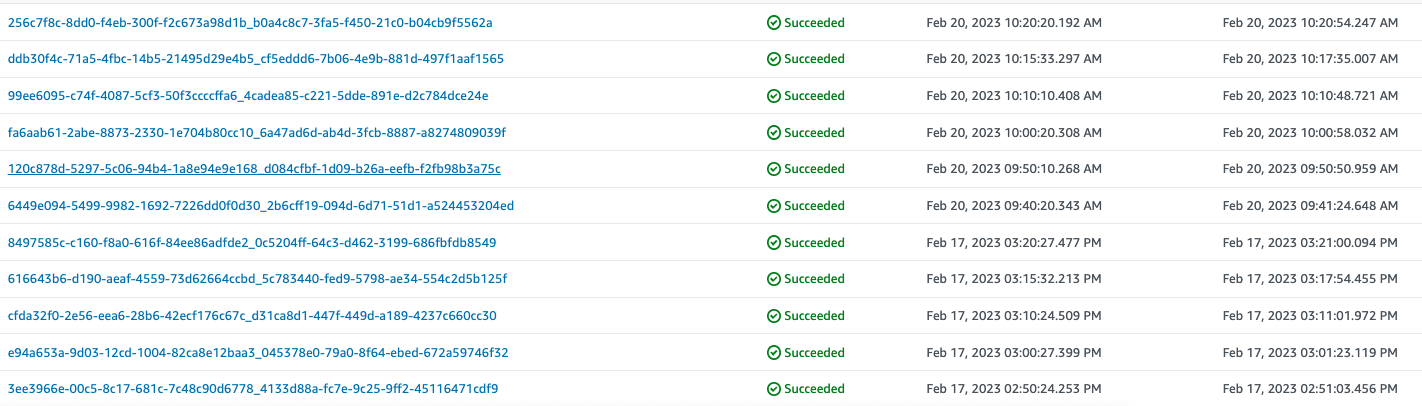
\includegraphics[width=15cm]{./diagrams/state_machine_cron_executions.png}
  \caption{State Machine Executions on a CRON }
 \end{figure}

 \section{Converting a CLI Test}
 Frankenstein also has a number of tests that test the functionality of the cli. The cli has most of the functionality if not more of the ServisBOT UI. The tests do not use a web scraper like Testcafe as it is not needed, instead the tests just run the cli commands and use an assertion to ensure they were carried out sufficiently. As a result the tests are completed much faster than the Testcafe tests.

The CLI test chosen was the Content, create-describe-update-delete-list test. It was a simple test that tests a Content node. It takes a content definition in JSON format and creates a content node object. Then it describes it, updates it, lists the contents and deletes the content. 
When deployed the test took 18 seconds as opposed to a Puppeteer test taking an average of 55 seconds.

When put to the team however, whether Bosco was to include CLI tests or not, it was agreed that it was unnecessary to include the CLI tests. Bosco was to test portal specifically where the users would 
be using the UI first hand. CLI tests were basically only for developers and there was less of a need to test them. The goal is to have full Frankenstein coverage with Bosco and testing the ServisBOT CLI proxy has 95\% coverage. 
It was then decided to remove the CLI test from Bosco. 

\section{Dynamo DB}
The next task for Bosco was to store the test results in a global Dynamo DB table. 
Each test run would have a row in the table with details on the results of the test. 
Initially the following attributes were chosen. The primary key was set to the test profile with the sort key which is unique set to the endTime of the test run. 
The other values passed to the dynamo table would be the duration of the test run and the status of the test run. Once the step function would write to the dynamo table, additional attributes would be added.

\begin{figure}[ht]
  \centering
  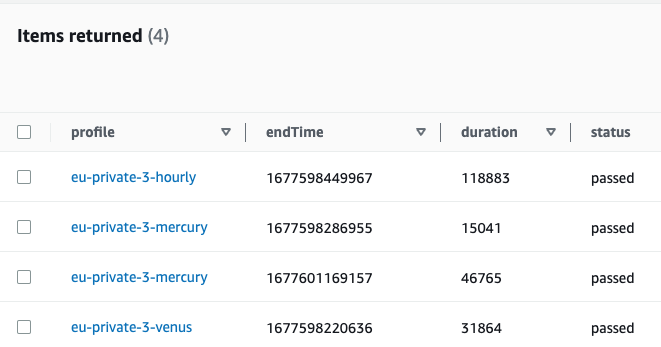
\includegraphics[width=15cm]{./diagrams/dynamodb.png}
  \caption{Dynamo DB Global Table Results}
 \end{figure}

The learning path to achieving this began with:
\begin{itemize}
\item Manually creating a dynamo table in dev and deciding the attributes that would be written to it.
\item The handler was then refactored in order to pass the profile, the endTime and the duration to the results lambda.
\item The results lambda then used the aws-sdk to write to the Dynamo DB. It filtered through the status of all the tests and if there was a failed test then the overall test run was marked as a fail.
\item Once the step function was writing to the table which was created manually, a new resource, a Global Dynamo table was added to the  CloudFormation template.
\item A condition was added to the Dynamo table so that it was possible to interchange between deploying the table or not.
\end{itemize}

\chapter{Deployment}
The deployment process was undertaken with help from the team as the initial plan needed to be altered. The triggers were removed from the 
 CloudFormation script and instead were put in a script specific to the AWS Region they would be deployed in. 

\section{CICD Process}
The steps to the CICD process for Bosco are as follows:

\begin{itemize}
  \item Developer puts in a PR (pull request) with the changes they made to the project code.
  \item Senior developer reviews the code and when ok, approves the merge.
  \item Developer merges branch which kicks off the CICD process. 
  \item Unit tests are run, artefacts are built and the project code is deployed on lower/staging/testing.
  \item If successful Slack will report on deployment, otherwise error needs to be located and debugged. 
  \item Developer tests the code changes on lower/staging/testing.
  \item When the changes are verified developer tags a release through deploybot on Slack.
  \item This initiates the CICD process again which builds artifacts, runs unit tests, integration tests and deploys to lower/staging/testing again as a tagged release.
  \item Developer tests on staging/lower/testing again.
  \item Once verified developer requests a deploy to production/testing from deploybot on Slack.
  \item CICD process is initiated once more with the project being deployed on production/upper.
  \item Developer tests the code on upper and verifies.
\end{itemize}

\section{Handling Multiple ServisBOT Regions}
It was required that Bosco would run multiple ServisBOT region test profiles per deploy. For example deploying an instance of 
Bosco in the AWS region, eu-west-1 should be capable of creating CRON schedules for ServisBOT regions, eu-1 and eu-private-1. 

\subsection{Triggers}
Triggers are what initiates the test runs. They can be defined for each region and each environment. The decision was taken 
to reduce the number of test runs that Frankenstein runs. Frankenstein runs 24/7 and this was deemed unnecessary. This will have a huge cost reduction 
effect on the company. The following times were decided on for the test runs.

\begin{table}[ht]
  \centering
  \small
  \setlength\tabcolsep{5pt}
  \begin{tabular}{|c|c|c|c|c|}
   \hline & \textbf{Staging/Lower}&\textbf{Prod/Upper}&\textbf{Prod/Upper}&\textbf{Prod/Upper}\\
   \hline\hline
   \textbf{ServisBOT Region}&\textbf{eu-private-1}&\textbf{eu-1}&\textbf{us1}&\textbf{usscif1}\\
   \hline
   \textbf{Timeframe}&Mon-Fri, 8am-5pm&24/7&24/7&24/7\\
   \hline
   \textbf{Mercury}&0,20,40&0,20,40&0,20,40&N/A\\
   \hline
   \textbf{Venus}&10,30,50&10,30,50&10,30,50&10,30,50\\
   \hline
   \textbf{Hourly}&hourly&hourly&hourly&hourly\\
   \hline
  \end{tabular}
  \caption{Scheduled Triggers (CRON)s for Running Bosco}
 \end{table}

A new folder src/triggers was created which contatins  CloudFormation templates for each AWS region and ServisBOT region pair.
For example:
src/triggers/eu-west-1/eu-1-triggers.yaml
src/triggers/eu-west-1/eu-private-1-triggers.yaml

Within each of these template files is the infrastructure for the eu-1 CRON and eu-private-1 respectively.
A new lambda was created in Bosco which does the following:
* When invoked, checks the AWS region the lambda is running in.
* Reads the src/triggers/<aws-region> folder, and uses the AWS SDK to deploy each of the templates found within this folder.
* The lambda function has the ability to poll to check for new or updated  CloudFormation stacks.
* The lambda will fail if any of the stacks fail to create/update.
A post-build code build script invokes the lambda. This now only runs on deployment to an account (not the CICD account).

\section{Additional Features Post-Deployment}

\subsection{Logging Test Results}
A new class was added, LogReporter in order to report the test results to Cloudwatch. Each test reports on itself plus each test run will log a completion report. 
These reports can be viewed in Cloudwatch in the following format.

\begin{figure}[H]
  \begin{tcolorbox}
   \begin{minted}{json}
    {
      "SbRegion": "eu-private-3",
      "TestProfile": "eu-private-3-venus",
      "TestTitle": "Bosco Interaction Test",
      "DurationInMs": 42268,
      "Result": "passed",
      "Type": "test",
      "TestRunnerIdentifier": "1b3bc8b5-7db5-48ae-83a4-3ad40a6bfa92"
  }
 \end{minted}
 \end{tcolorbox}
 \captionof{figure}{Cloudwatch Log of Bosco Interacton Test}
 \end{figure}

 \begin{figure}[H]
  \begin{tcolorbox}
   \begin{minted}{json}
    {
      "SbRegion": "eu-private-3",
      "TestProfile": "eu-private-3-venus",
      "TotalDurationInMs": 120218,
      "Result": "passed",
      "Type": "completion",
      "TestRunnerIdentifier": "1b3bc8b5-7db5-48ae-83a4-3ad40a6bfa92"
  }
 \end{minted}
 \end{tcolorbox}
 \captionof{figure}{Cloudwatch Log of Complete Test Run}
 \end{figure}

 \subsection{Cloudwatch Insights}
 A query was constructed and added to the READMe to make it easier for developers to be able to view failed test results.
 The following figure is the result of the query. 
 \begin{figure}[ht]
  \centering
  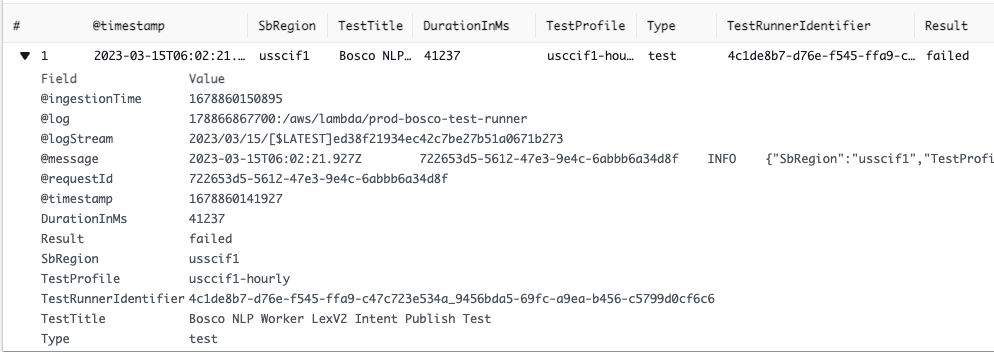
\includegraphics[width=\textwidth,height=\textheight,keepaspectratio]{./diagrams/insights.png}
  \caption{Cloudwatch Log Insight of Failed Tests for 1 week on Production}
 \end{figure}

\subsection{Failed Test Screenshots stored in S3}
On failure of a test, a screenshot is taken using Puppeteer and stored locally in a /tmp/screenshots folder with the execution ID of the state 
machine run. On completion of the test run, the handler checks for the existance of a directory with the execution ID and if 
it exists then it runs through each file in the directory which will be a screenshot of the moment the test failed and it uploads 
these screenshots to an S3 bucket. The /tmp directroy is the only directory that lambda can access. Any attempts to read/write 
to other named directories will cause an error. Once the files have been uploaded the /tmp/screenshots directory is deleted.

The S3 bucket is deployed using  CloudFormation. There is a condition on the bucket to deploy only in a staging environment and 
otherwise only if specified. Cloudformation permissions were added to allow for upload to the specific bucket.

The process to achieving this feature began initially with each test storing the screenshot on a failure. A new function 
was written in the Lightning Page class
\begin{figure}[ht]
  \centering
  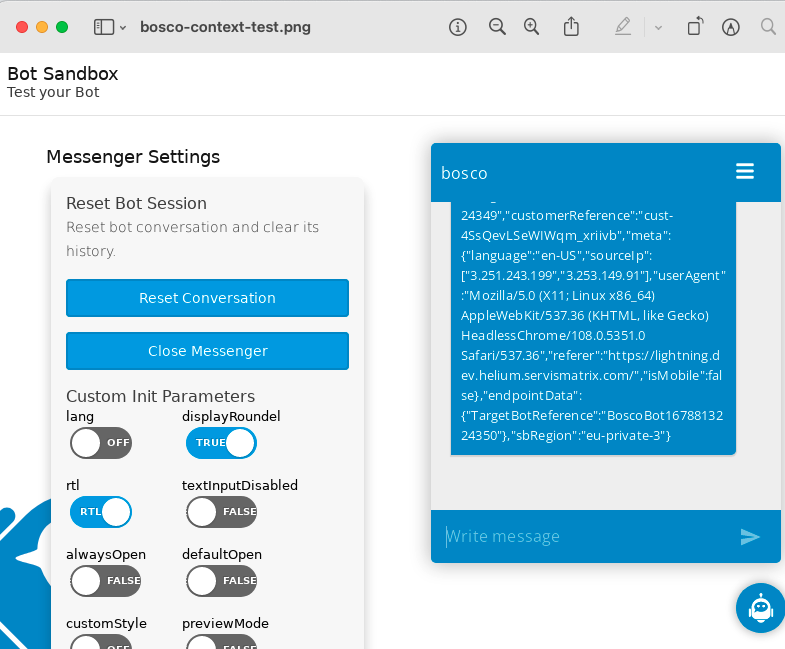
\includegraphics[width=\textwidth,height=\textheight,keepaspectratio]{./diagrams/screenshot.png}
  \caption{Screenshot of failed test}
 \end{figure}

\chapter{Conclusion}
\section{Reflection}
\section{Key skills}
\begin{itemize}
  \item Sprint planning. 
  \item Amazon Web services, in particular Lambda, Step Functions, § CloudFormation, S3, DynmaoDB, AWS regions, SSM Parameters, 
  \item Showcasing progress of the project to the team
  \item LateX
  \item CICD process
  \item Git
  \item Javascript fundamentals
  \item Project design and infrastructure 
  \item Puppeteer and Mocha
  \item Docker
\end{itemize}
\section{Challenges}
Fortunately the team at ServisBOT were very supportive and as a result, working on this project posed very few challenges. However, there 
were a few which may be common to work based projects for students completing theirs in the workplace.
\begin{itemize}
  \item It became obvious early in the process that the fundamentals of Javascript and object orientated programming was still challenging and not fully comprehended by myself. However, from being tasked with new problems every day and week, which explored 
  varioius components, AWS services, features and technologies, an immense learning curve was accomplished and skills achieved at a pace which inevitably sped up the process by the week.
  \item As this was a work based project which was completed during an internship, the code had to be reviewed by a team member before being merged into the main branch. If the team was under pressure this could take a few days which disrupted the workflow.
  \item Learning how to use LateX for the project report initially was very confusing and stunted the process. It was almost as challenging as learning a new programming language yet the benefits from using it outweighed the frustrations.
\end{itemize}

\section{Future Work}
Incredibly at the end of the project, Bosco is at a state where the team can now take over and add the remainder of the tests. There are about forty tests that are to be transitioned from Frankenstein to Bosco which any team member 
once lightly versed in Puppeteer and Mocha can work on easily. 

\appendix
\chapter{Methodology}
Jira was used to keep track the sprints on the Bosco project. Week long sprints were the chosen method for the implementation phase as this
was better suited to the type of project as the urgency to have it complete is high.

The projcet was broken into three Epics:

\begin{itemize}
  \item Bosco Research and Design
  \item Bosco Implementation
  \item Bosco Dissemination Phase
\end{itemize}
\section{Research and Design}
Research and Design was carried out over a number of weeks starting in December with the main focus on the following:
\begin{itemize}
\item Review Puppeteer
\item Review Lambda
\item Initial Step Function R\&D
\item Cost Analysis
\end{itemize}

\section{Implementation}
The implementation of Bosco was carried out in one week sprints as was required by the project supervisor in ServisBOT\@. 
\subsection*{Sprint 1}
\begin{itemize}
\item Add two Frankenstein tests to Bosco
\item Step Function Lambda code moved to Bosco
\end{itemize}

\subsection*{Sprint 2}
\begin{itemize}
\item Cloudformation
\end{itemize}

\subsection*{Sprint 3}
\begin{itemize}
\item Bosco environment variables for tests
\item Refactor state machine to use a shared environment
\end{itemize}

\subsection*{Sprint 4}
\begin{itemize}
\item Test profiles and overrides
\end{itemize}

\subsection*{Sprint 5}
\begin{itemize}
\item Create a test with a secret
\end{itemize}

\subsection*{Sprint 6}
\begin{itemize}
\item Lightning url in tests needs to be config in test profiles
\end{itemize}

\subsection*{Sprint 7}
\begin{itemize}
\item READMe update for Developer Experience
\item Schedule different test profiles to run on a CRON
\item Orchestrator builds the Environment
\end{itemize}

\subsection*{Sprint 8}
\begin{itemize}
\item Create a CLI test in Bosco
\item Staging organization and SSM Parameters
\end{itemize}

\subsection*{Sprint 9}
\begin{itemize}
\item Deployment of Bosco
\item Storing Test Results in Dynamo DB
\item Logging Test Results and Completion
\item Bosco infrastructure to handle multiple ServisBOT regions with one deploy
\end{itemize}

\subsection*{Sprint 10}
\begin{itemize}
\item Screenshots of failed tests upload to S3
\item Alert of test failures and failed test runs
\end{itemize}

\begin{figure}[ht]
 \centering
 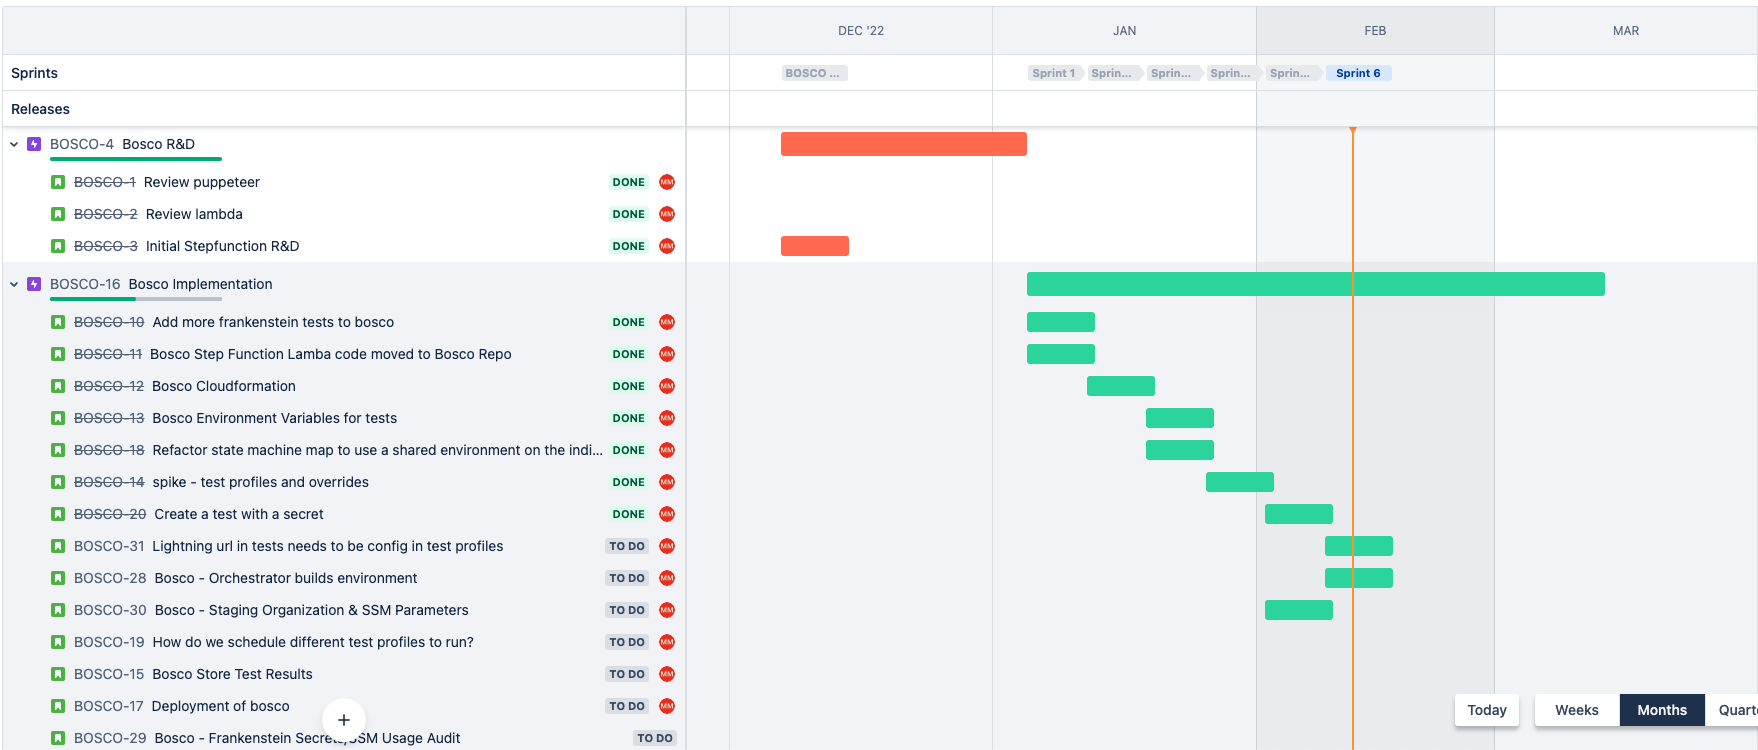
\includegraphics[width=15cm]{./diagrams/sprints1.png}
 \caption{R\&D Phase and Bosco Implementation Phase}
\end{figure}

\begin{figure}[ht]
 \centering
 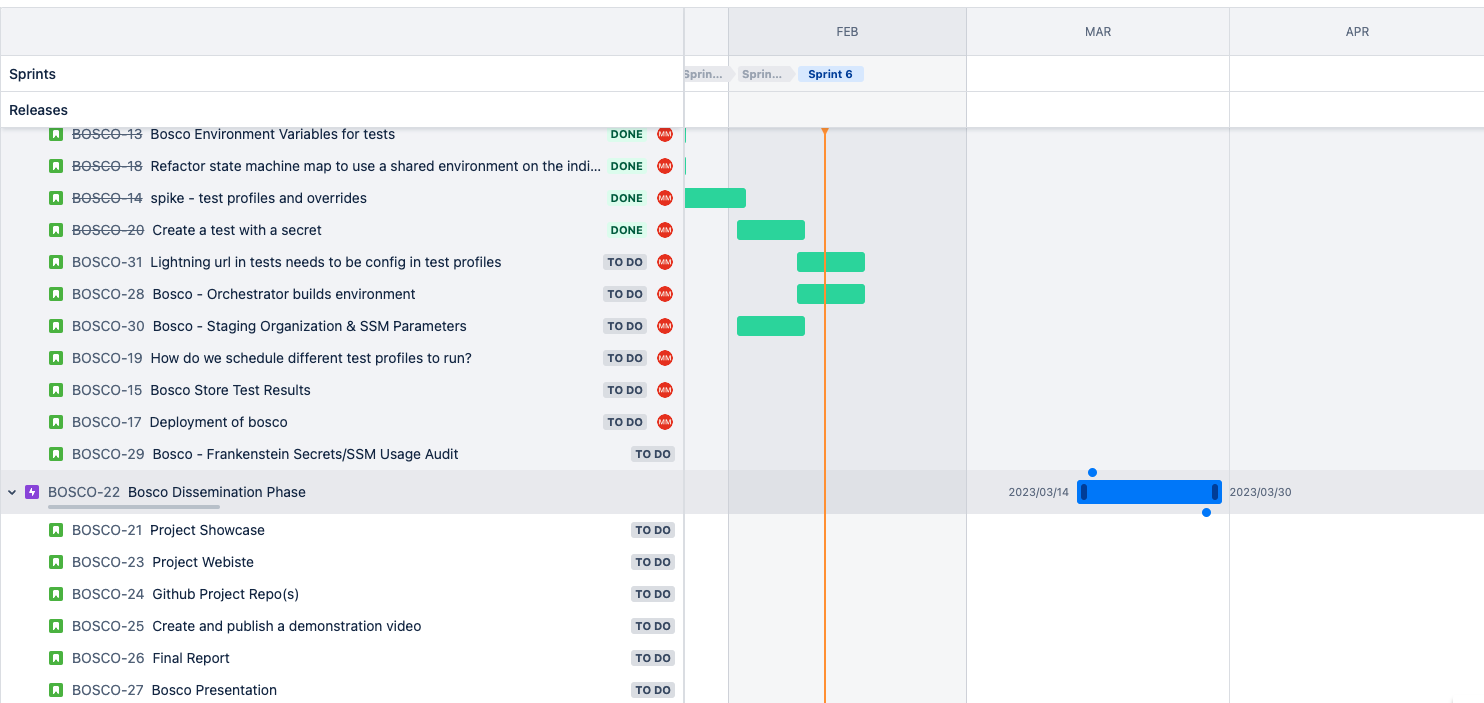
\includegraphics[width=15cm]{./diagrams/sprints2.png}
 \caption{Bosco Dissemination Phase}
\end{figure}

\chapter{Dependencies and Dev-Dependencies}
\subsection*{dependencies}
\textbf{@aws-sdk/client-dynamodb}
\textbf{@aws-sdk/lib-dynamodb}
\textbf{@servisbot/servisbot-cli}
\textbf{bluebird}
\textbf{cors}
\textbf{csv-parse}
\textbf{express}
\textbf{loglevel} was added to replace the console.logs.
\textbf{luxon}
\textbf{number-to-words-en}
\textbf{puppeteer}
\textbf{serverless-http}
\textbf{sinon}
\textbf{supertest}

\subsection*{dev-dependencies}
\textbf{aws-sdk}
\textbf{depcheck}: a dependency check package which checks for unused dependencies before commits.
\textbf{eslint}: a linting tool that ensures all the code is formatted consistently by anyone who makes changes to the code.
\textbf{lambda-local}, a node module was used for testing purposes. This allowed for the running of the lamdas locally rather than having 
to deploy each time they were to be tested. 
\textbf{mocha}
\textbf{pre-commit}

\begin{figure}[ht]
  \centering
  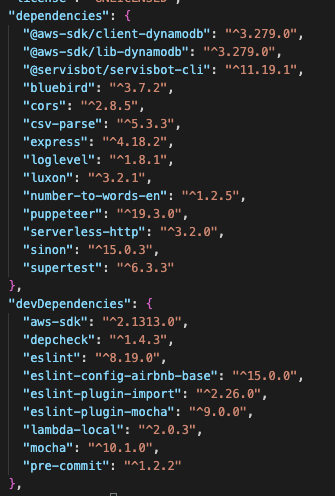
\includegraphics[width=15cm]{./diagrams/dependencies.png}
  \caption{dependencies and dev dependencies used for Bosco}
 \end{figure}

\printbibliography[title={References}]

\chapter{Bibliography}
\begin{enumerate}
\item https://www.opsramp.com/guides/aws-monitoring-tool/cloudwatch-synthetics/
\item https://www.functionize.com/automated-testing/assertion
\item https://jestjs.io
\item https://www.browserstack.com/guide/unit-testing-for-nodejs-using-mocha-and-chai
\item https://www.tricentis.com/blog/bdd-behavior-driven-development
\item https://www.pluralsight.com/blog/software-development/tdd-vs-bdd
\item https://www.testim.io/blog/puppeteer-selenium-playwright-cypress-how-to-choose/
\item https://www.testim.io/blog/webinar-summary-is-ai-taking-over-front-end-testing/
\item https://aws.amazon.com/blogs/architecture/field-notes-scaling-browser-automation-with-puppeteer-on-aws-lambda-with-container-image-support/
\item https://moiva.io/
\item https://docs.aws.amazon.com/AmazonCloudWatch/
\item https://docs.aws.amazon.com/lambda/latest/dg/gettingstarted-limits.html
\item https://oxylabs.io/blog/puppeteer-on-aws-lambda
\item https://aws.amazon.com/blogs/aws/new-for-aws-lambda-container-image-support/
\item https://www.npmjs.com/package/chrome-aws-lambda
\item https://www.docker.com/resources/what-container/
\item https://blog.logrocket.com/testing-node-js-mocha-chai/
\item https://www.ponicode.com/shift-left/
\item https://blog.shikisoft.com/3-ways-to-schedule-aws-lambda-and-step-functions-state-machines/
\item https://evanhalley.dev/post/aws-ssm-node/
\item https://dockerlabs.collabnix.com/beginners/components/what-is-container.html
\item https://www.youtube.com/watch?v=rQijrDj1wCQ
\end{enumerate}

\end{document}